\documentclass{standalone}
\usepackage{tikz}
\begin{document}

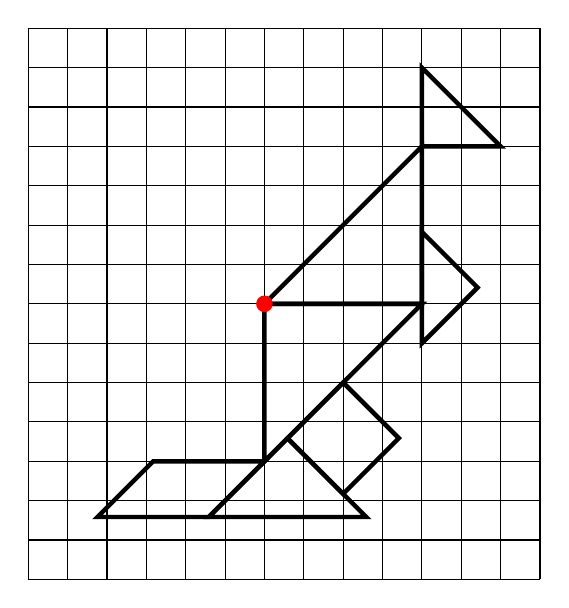
\begin{tikzpicture}
\draw[step=5mm] (-3.0, -3.5) grid (3.5, 3.5);
\draw[ultra thick] ({2}, {3}) -- ({3}, {2}) -- ({2}, {2}) -- cycle;
\draw[ultra thick] ({2}, {2}) -- ({2}, {0}) -- ({0}, {0}) -- cycle;
\draw[ultra thick] ({2}, {-1/2+sqrt(2)}) -- ({2+1/2*sqrt(2)}, {-1/2+1/2*sqrt(2)}) -- ({2}, {-1/2}) -- cycle;
\draw[ultra thick] ({0}, {0}) -- ({2}, {0}) -- ({0}, {-2}) -- cycle;
\draw[ultra thick] ({1}, {-1}) -- ({1+1/2*sqrt(2)}, {-1-1/2*sqrt(2)}) -- ({1}, {-1-sqrt(2)}) -- ({1-1/2*sqrt(2)}, {-1-1/2*sqrt(2)}) -- cycle;
\draw[ultra thick] ({1-1/2*sqrt(2)}, {-1-1/2*sqrt(2)}) -- ({2-1/2*sqrt(2)}, {-2-1/2*sqrt(2)}) -- ({-1/2*sqrt(2)}, {-2-1/2*sqrt(2)}) -- cycle;
\draw[ultra thick] ({-sqrt(2)}, {-2}) -- ({0}, {-2}) -- ({-1/2*sqrt(2)}, {-2-1/2*sqrt(2)}) -- ({-3/2*sqrt(2)}, {-2-1/2*sqrt(2)}) -- cycle;
\fill[red] (0,0) circle (3pt);
\end{tikzpicture}

\end{document}
